% beautiful title slides in Beamer
% Model 6
% latex-beamer.com

\documentclass[aspectratio=169]{beamer}

\usepackage{media9}
\usepackage[backend=bibtex, style=authoryear, doi=false,isbn=false,url=false]{biblatex}
\usepackage[most]{tcolorbox}
\usepackage{subcaption}
\usepackage{bm}
\usepackage{diffcoeff}

% Math macros
\renewcommand\d{\ensuremath{\mathrm{d}}}

\DeclareMathOperator*{\grad}{grad}
\DeclareMathOperator*{\Grad}{Grad}
\DeclareMathOperator*{\Div}{Div}
\renewcommand{\div}{\operatorname{div}}

\newcommand{\bbR}{\mathbb{R}}
\newcommand{\bbF}{\mathbb{F}}
\newcommand{\bbA}{\mathbb{A}}
\newcommand{\bbB}{\mathbb{B}}
\newcommand{\bbS}{\mathbb{S}}

\DeclareMathOperator{\tr}{tr}

\newcommand*{\dual}[1]{\ensuremath{\widehat{#1}}}
\newcommand*{\norm}[1]{\ensuremath{\left\|#1\right\|}}
\newcommand{\where}{\qquad \text{where} \qquad}

\newcommand{\inpr}[3][]{\ensuremath{( #2, \, #3 )_{#1}}}
\newcommand{\dualpr}[3][]{\ensuremath{\langle #2 \, \vert #3 \rangle_{#1}}}

\newcommand{\pder}[2]{\ensuremath{\partial_{#2} #1}}
\newcommand{\dder}[2]{\ensuremath{\delta_{#2} #1}}

% Remove navigation bar
%\setbeamertemplate{navigation symbols}{}
\addtobeamertemplate{navigation symbols}{}{%
	\usebeamerfont{footline}%
	\usebeamercolor[fg]{footline}%
	\hspace{1em}%
	\insertframenumber/\inserttotalframenumber
}

\usepackage{color}
\definecolor{theme}{RGB}{0,73,114}

\setbeamertemplate{blocks}[rounded][shadow]

\setbeamercolor{block body alerted}{bg=alerted text.fg!10}
\setbeamercolor{block title alerted}{bg=alerted text.fg!20}
\setbeamercolor{block body}{bg=structure!10}
\setbeamercolor{block title}{bg=structure!20}
\setbeamercolor{block body example}{bg=green!10}
\setbeamercolor{block title example}{bg=green!20}
% Tikz package
\usepackage{tikz}
\usetikzlibrary{positioning}




\graphicspath{{./images/}}

\bibliography{biblio}


%% At begin of each section: show current section and all subsections in the section if any
%% At begin of each subsection except first: show only the current section/subsection
\newif\iftocsub
\tocsubtrue
\AtBeginSection[] {
	\begin{frame}[noframenumbering]{Outline}
		\tableofcontents[sectionstyle=show/shaded, subsectionstyle=show/show/hide]
	\end{frame}
	\tocsubfalse
}
\AtBeginSubsection[] {
	\iftocsub
	\begin{frame}[noframenumbering]{Outline}
		\tableofcontents[currentsubsection, sectionstyle=show/shaded, subsectionstyle=show/shaded/hide]
	\end{frame}
	\fi
	\tocsubtrue
}

\newcommand{\beginbackup}{
	\newcounter{framenumbervorappendix}
	\setcounter{framenumbervorappendix}{\value{framenumber}}
}
\newcommand{\backupend}{
	\addtocounter{framenumbervorappendix}{-\value{framenumber}}
	\addtocounter{framenumber}{\value{framenumbervorappendix}} 
}

\begin{document}
	
	
	
	
	% Title slide frame
	\begin{frame}[plain]
		
		%%%%%%%% Title slide details %%%%%%%%%%%%%%


% Background Image
\newcommand{\myBackground}
{
    
\includegraphics[height=1.02\paperheight,page=9]{beamerthemeutresources}
}

% Title
\newcommand{\myTitle}
{
    Numerics for the Portwings project
}

% Subtitle
\newcommand{\mySubTitle}
{
    Current develpments and outlook
}

% Author
\newcommand{\myAuthor}   
{
    Andrea Brugnoli
}

% Affiliation
\newcommand{\myAffiliate}
{
  
}

% Presentation Date
\newcommand{\myDate}   
{
    \today
}

% Logo
\newcommand{\myLogo}   
{
    
\includegraphics[width=3cm]{Logo.png}
}
%%%%%%%%%%%%%%%%%%%%%%%%%%%%%%%%%%%%


%%%%%%%%%% Title slide code %%%%%%%%%%%
\begin{tikzpicture}[remember picture,overlay]

% Background color

\fill[white] (current page.south west) rectangle (current page.north east);
% Background image
\node[above right,inner sep=0pt] at (current page.south west)
    {
        \myBackground
    };
    
% Title & Subtitle
\node
[
    above=0.5cm,
    align=center,
    draw=black!50,
    % rounded corners,
    double,
    double distance=0.1cm,
    double=blue!10,
    fill=yellow!10,
    inner xsep=15pt,
    inner ysep=10pt, 
    minimum width=0.7\textwidth,
    text width=0.6\textwidth
] (title) at (current page.center)
{
    \LARGE \myTitle  \\[5pt]
    \small \mySubTitle
};

% Author 
\node[ below=0.5cm] (author) at (title.south){\myAuthor};

% Author 
\node[ below=0.25cm ](affiliate) at (author.south){\small \myAffiliate};

% Date
\node[below=0.25] (date) at (affiliate.south){\large \myDate};

% Logo
\node
[
    below =0.25cm
] at (date.south)
{
    \myLogo
};

\end{tikzpicture}
		
	\end{frame}
	
	\begin{frame}{Overview}
		\tableofcontents
	\end{frame}
	
	\section{The reason behind my research}
	
	\begin{frame}{Motivation: multiphysics problems}
		
		Multiphysics problems are commonly found in industrial applications.
		\begin{figure}[t]
			\begin{subfigure}[t]{0.34\textwidth}
				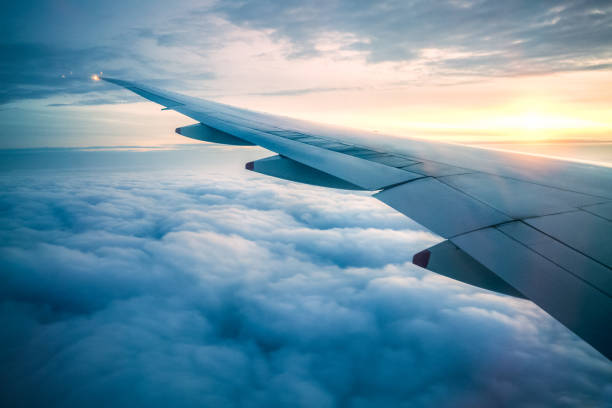
\includegraphics[width=\columnwidth]{wing.jpg}\\
				\centering{Aeroelasticity}%
			\end{subfigure}\hfill
			\begin{subfigure}[t]{0.3\textwidth}
				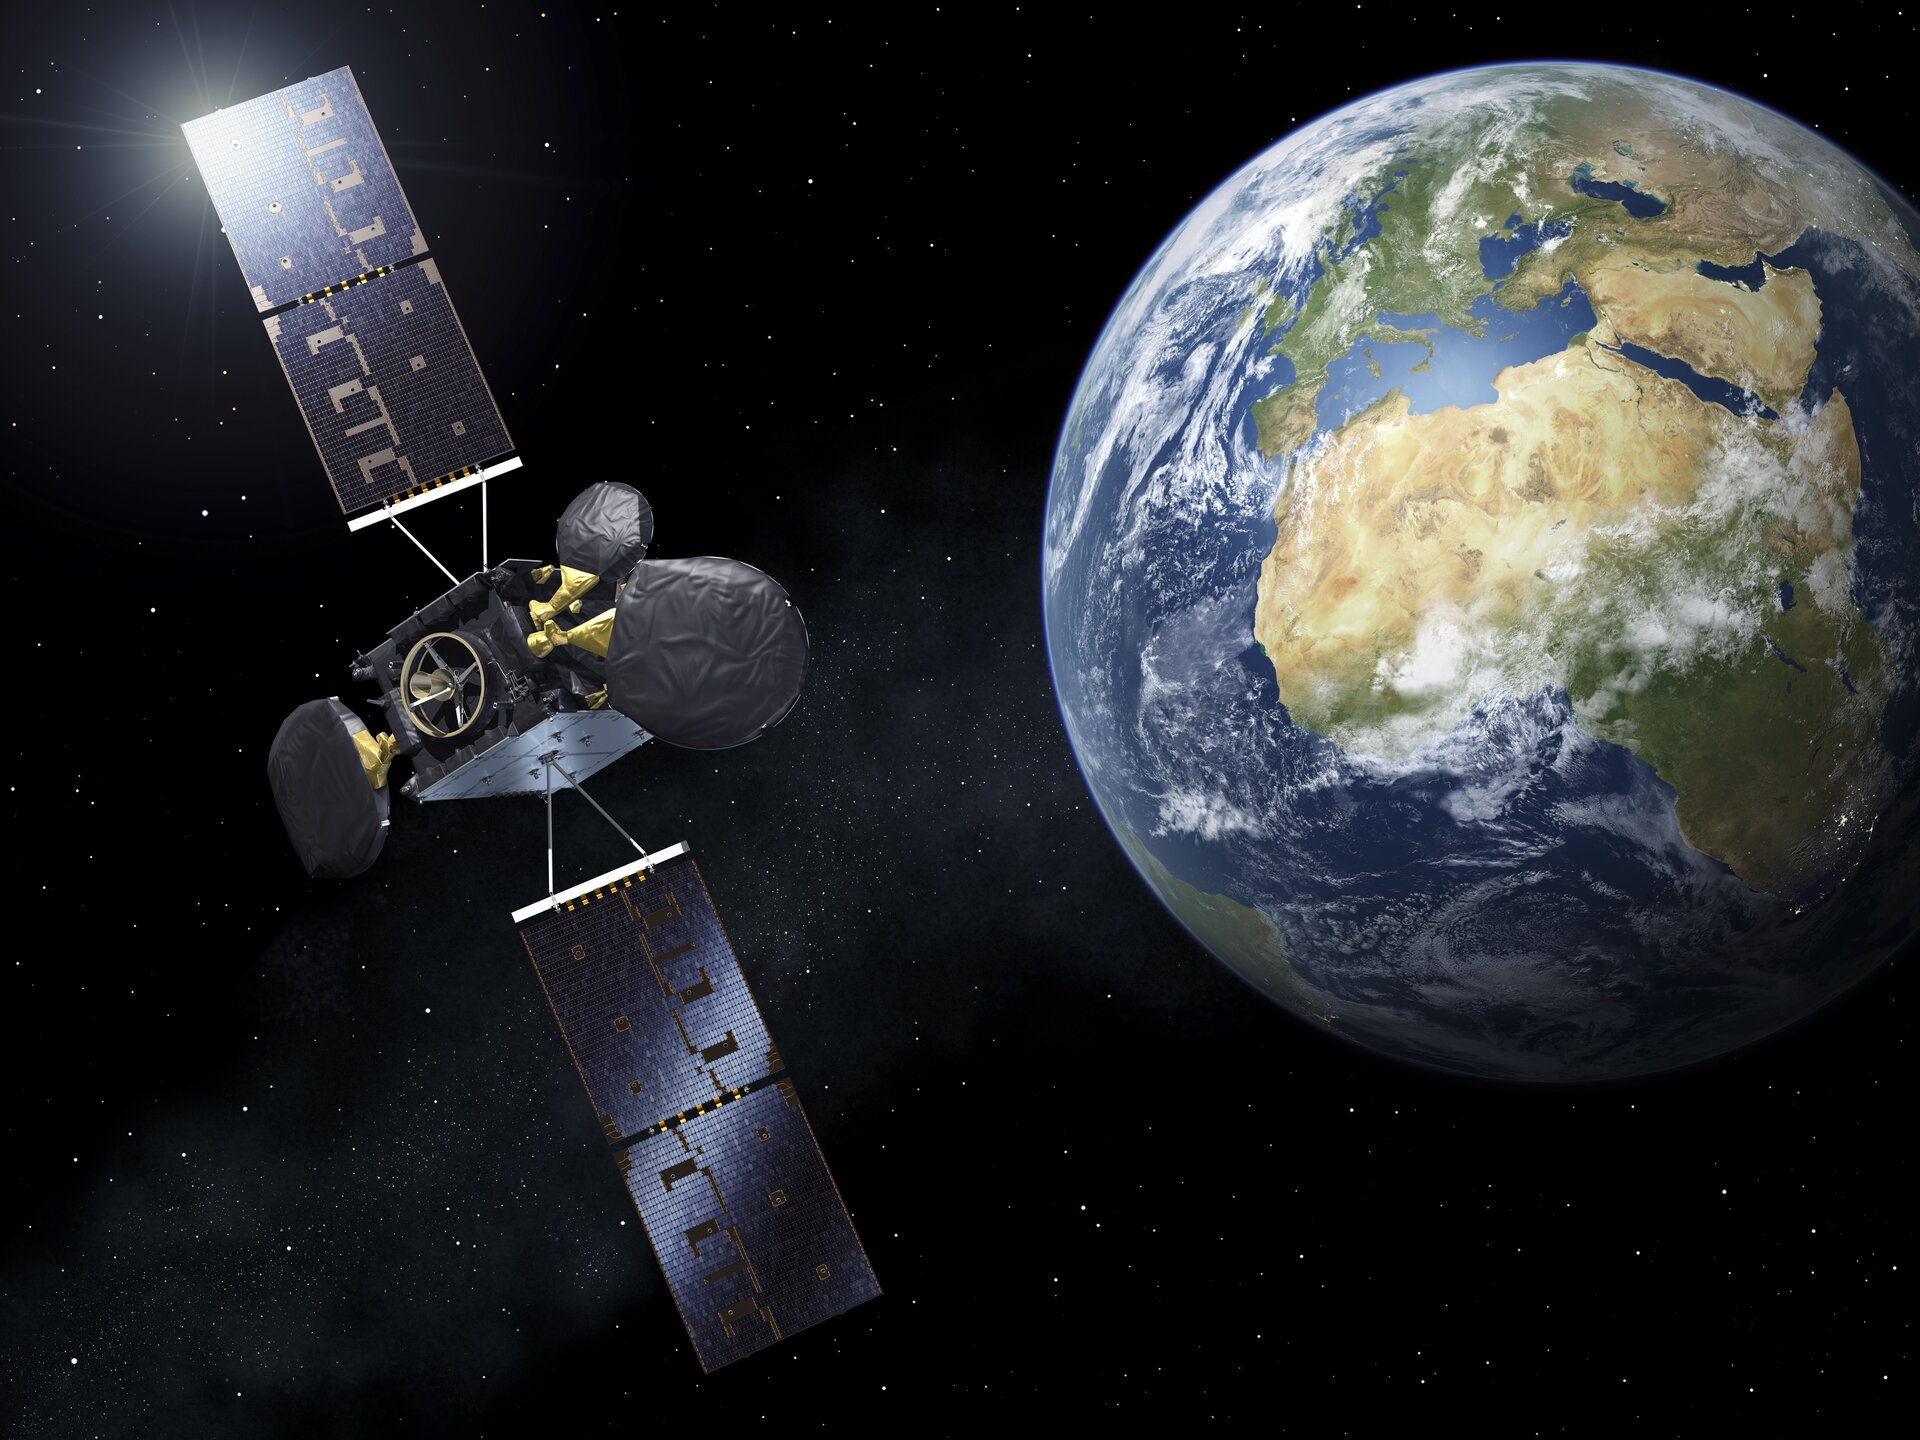
\includegraphics[width=\columnwidth]{esa_satellite.jpg}\\
				\centering{Thermoelasticity} 
			\end{subfigure}\hfill
			\begin{subfigure}[t]{0.26\textwidth}
				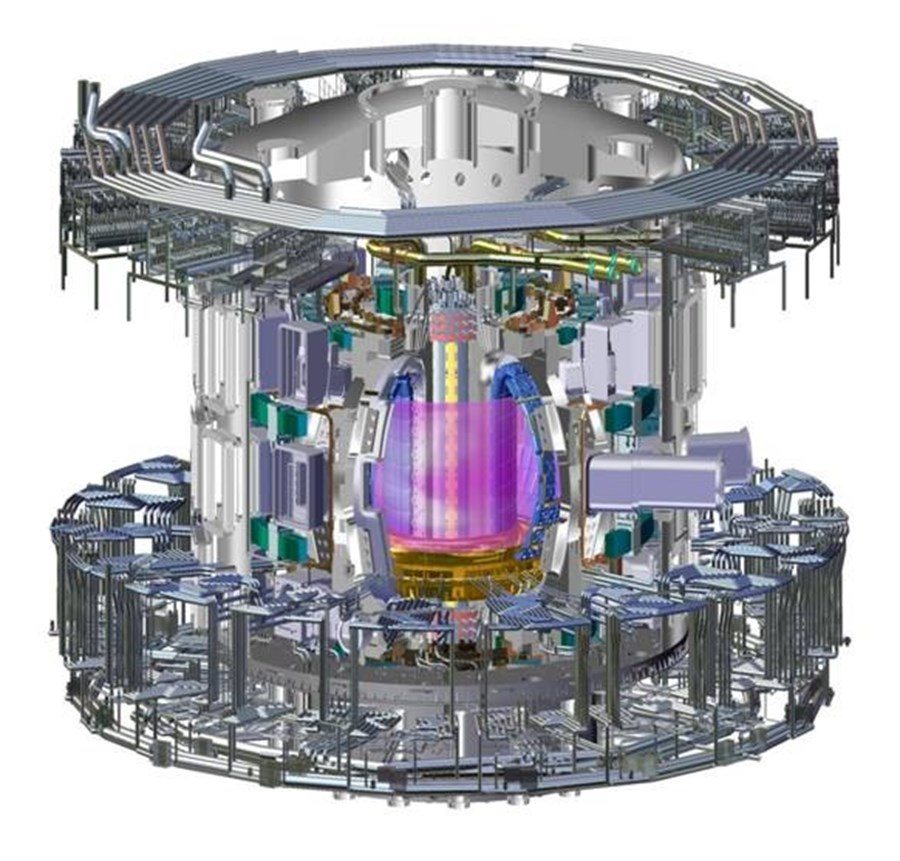
\includegraphics[width=\columnwidth]{tcws.jpg}\\
				\centering{Magnetohydrodynamics}
			\end{subfigure}
		\end{figure}
		Challenges:
		\begin{itemize}
			\item Coupling between different models.​
			\item Huge computational cost due to the large size of the models.​
			\item Multidisciplinary optimization for dynamical systems.​
		\end{itemize}
		
	\end{frame}

	\begin{frame}{Typical workflow in industry}
		
		\begin{itemize}
			\item \textbf{Specific modelling} and numerical methods for each physical domain. 
			\begin{itemize}
				\item[$-$] The \textbf{open character} of systems is \textbf{not considered}.
				\item[$-$] \textbf{Physical interconnection} of systems is not properly accounted for.
			\end{itemize}
			\item Model reduction via statistical methods.
			\begin{itemize}
				\item[$-$] The \textbf{physical structure is lost} and first principles are violated.
				\item[$-$] This methodology \textbf{does not generalize} to different problems.
			\end{itemize}
			\vspace{.3cm}
			\begin{figure}[t]
				\centering
				\begin{subfigure}[t]{0.4\textwidth}
					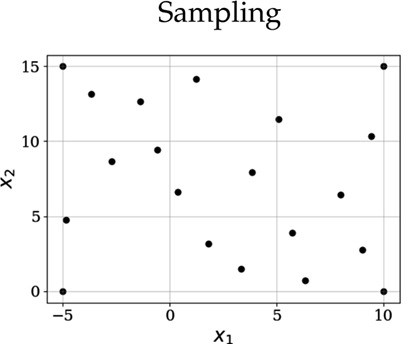
\includegraphics[width=.8\columnwidth]{sampling.jpg}
				\end{subfigure}\hspace{1cm}
				\begin{subfigure}[t]{0.4\textwidth}
					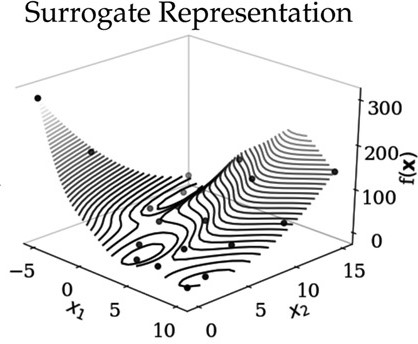
\includegraphics[width=.8\columnwidth]{surrogate_model.jpg}
				\end{subfigure}
			\end{figure}
		\end{itemize}
	\end{frame}
	
	
	\begin{frame}{Vision for the portwings project}
		
		\begin{block}{Main objective}
			Use a unified port-Hamiltonian (pH) framework to model fluid-structure interactions.
		\end{block}
		
		
		\begin{figure}[t]
				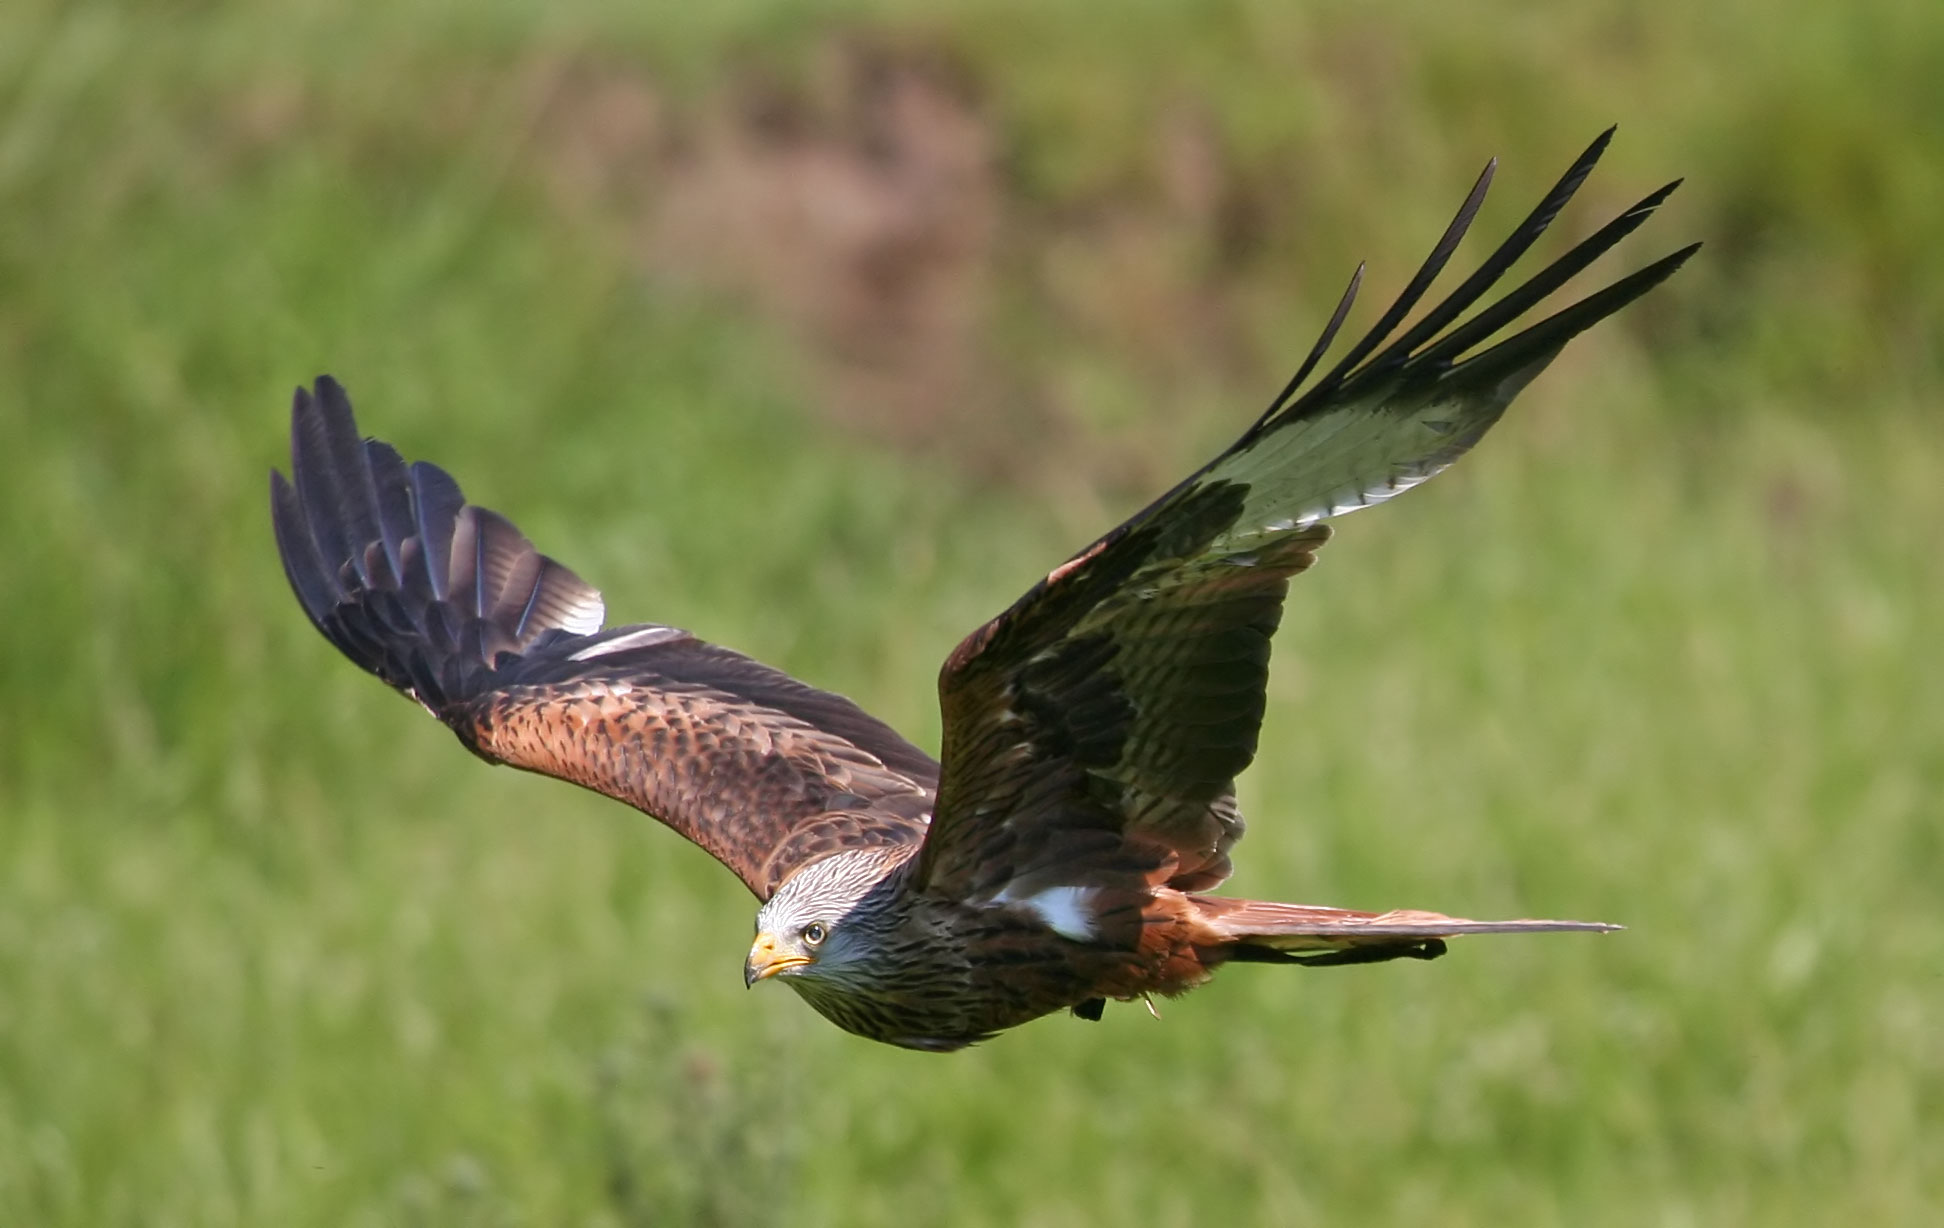
\includegraphics[width=.5\columnwidth]{Flying_Falcon.jpg}\\
		\end{figure}
		
		
	\end{frame}
	
	
	\begin{frame}{A unified language for multiphysics in engineering}
		Main features of port-Hamiltonian (pH) systems:
		\vspace{.1cm}
		\begin{columns}
			\begin{column}{.65\textwidth}
				\begin{itemize}
					\item \textbf{Physics} is at the \textbf{core}: pH systems are \textbf{passive} with respect to the \textbf{energy storage function}.
					\item Separation of \textbf{topology} and \textbf{metric} .
					\item PH systems are \textbf{closed under interconnection}. 
				\end{itemize}
			\end{column}
			\begin{column}{.35\textwidth}
				\centering
				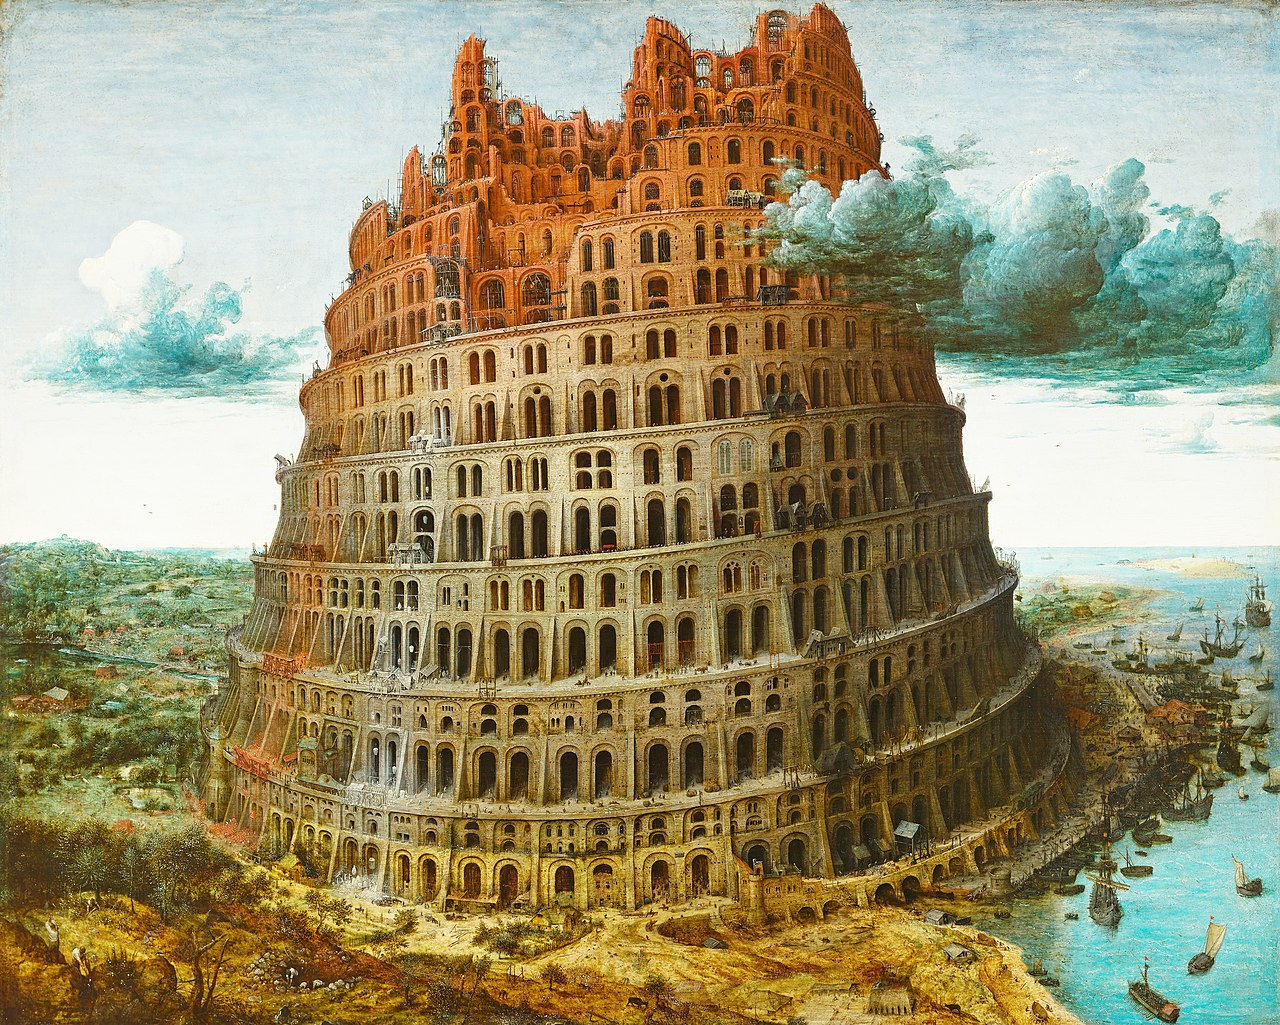
\includegraphics[width=.9\columnwidth]{babel_tower.jpeg}
			\end{column}
		\end{columns}
	\end{frame}

\begin{frame}{Physics}
	
	\begin{columns}
		\begin{column}{.5\textwidth}
			\begin{figure}
			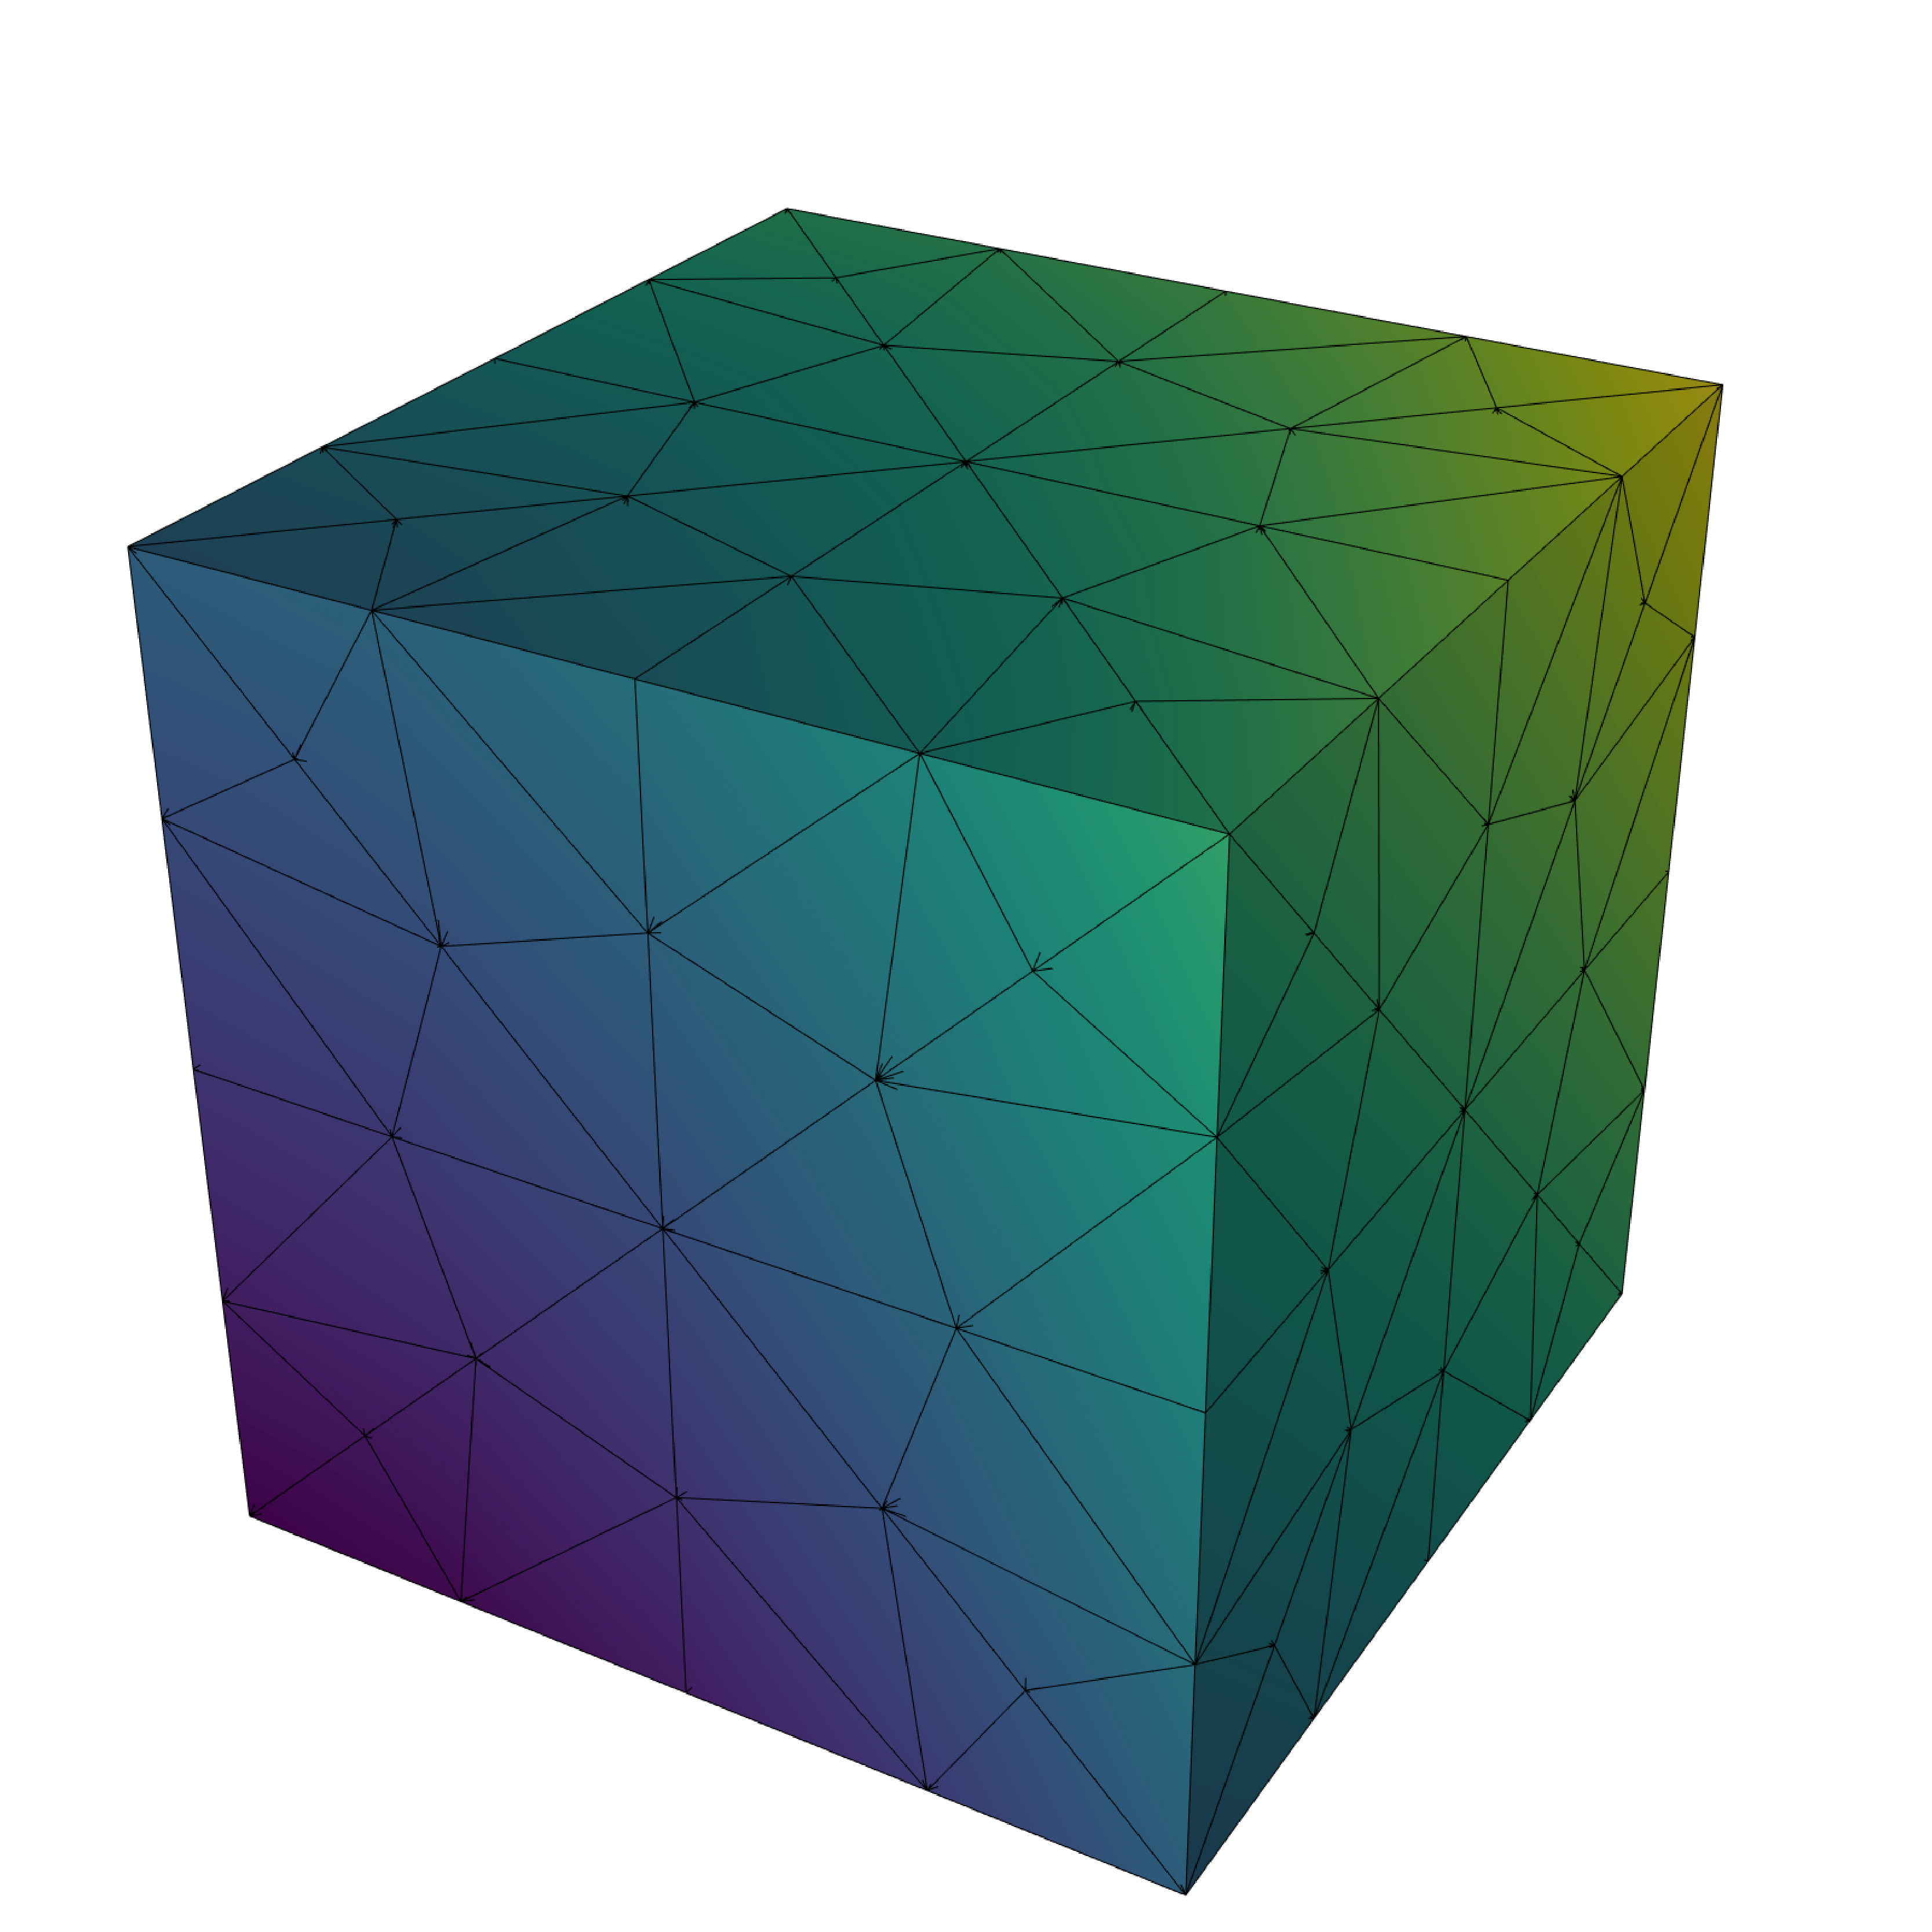
\includegraphics[width=.95\columnwidth]{cube_sol.pdf}
			\caption*{Temperature in a cube}
			\end{figure}
			\end{column}
		
		\begin{column}{.5\textwidth}
			\begin{equation*}
				\begin{aligned}
				\partial_t \theta &= \Delta \theta, \\
				U(t) &= \theta(t), \qquad \qquad \text{Energy}, \\
				S(t) &= \log \theta(t), \qquad\; \text{Entropy}. \\
				\end{aligned}
			\end{equation*}
		\vspace{1cm}
		\begin{equation*}
			\begin{aligned}
				\diff{U}{t} &=\int_{\partial \Omega} \diffp{\theta}{\bm{n}} \d\Sigma, \\
				\diff{{S}}{t} &= \int_{\Omega} \frac{||\grad \theta||^2}{\theta^2} \d\Omega + \int_{\partial\Omega}\frac{1}{\theta} \diffp{\theta}{\bm{n}} \d\Sigma. \\
			\end{aligned}
		\end{equation*}
		Numerical methods need to respect physics
		\end{column}
	\end{columns}
	
	
	\end{frame}

\begin{frame}{Metric and topology}
	\begin{columns}
		\begin{column}{.5\textwidth}
				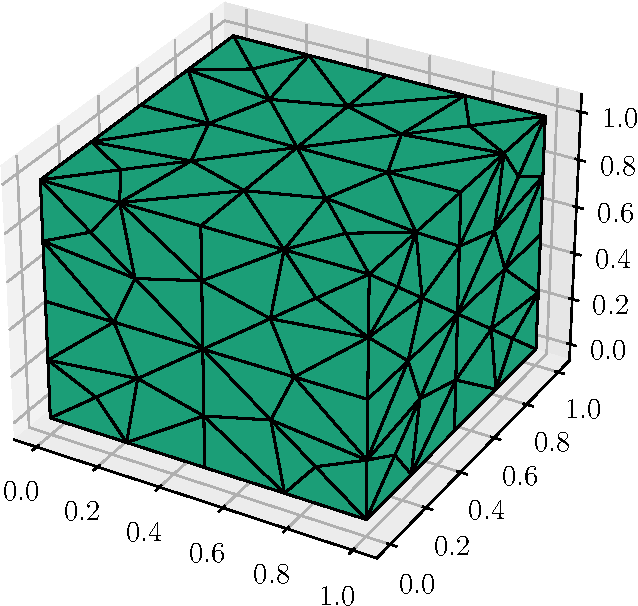
\includegraphics[width=.9\columnwidth]{mesh_cube.pdf}
		\end{column}
	\begin{column}{.5\textwidth}
		\includegraphics[width=.9\columnwidth]{topology.eps}
		\vspace{1cm}
	\end{column}
	\end{columns}

\end{frame}

\begin{frame}{Interconnection of port-Hamiltonian systems}
	\only<1>{
		\begin{figure}
			\centering
			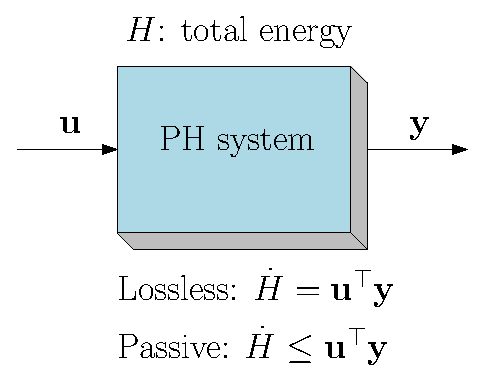
\includegraphics[width=.6\textwidth]{sketch_PH.eps}
		\end{figure}
			}
	\only<2>{
		\begin{figure}
			\centering
			\includegraphics[width=.95\textwidth]{sketch_PH_gyrator.eps}
		\end{figure}
	}
	\only<3>{
		\begin{figure}
			\centering
			\includegraphics[width=.95\textwidth]{sketch_PH_transformer.eps}
		\end{figure}
	}
\end{frame}


	
	\section{Some examples}
	
	
	\begin{frame}{Rigid rod welded to a cantilever plate}
		\only<1>{
		\begin{figure}
			\centering
			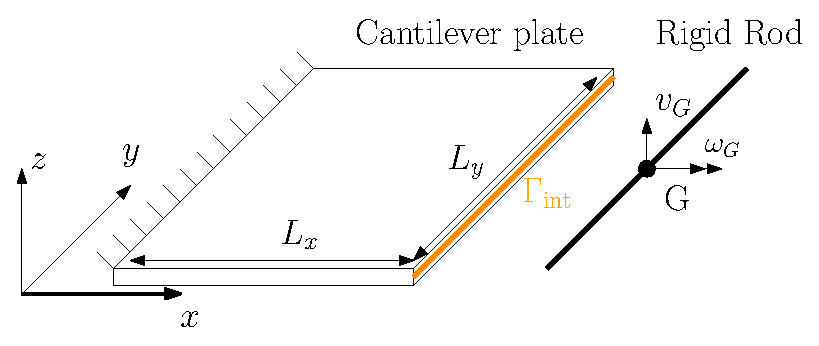
\includegraphics[height=0.3\textheight]{plate_rod_separated.eps}\\
			\vspace{1cm}
			\includegraphics[height=0.3\textheight]{plate_rod_welded.eps}
		\end{figure}
		}
		\only<2>{
			\centering 
		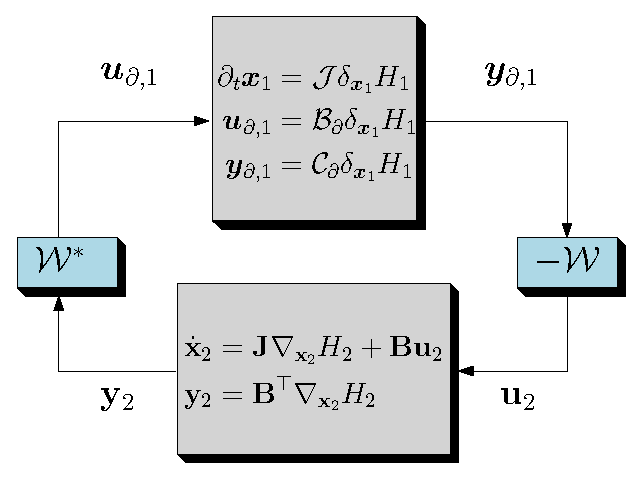
\includegraphics[width=0.48\textwidth]{pp_interconnection.eps}
		\hspace{5pt}
		\includegraphics[width=0.48\textwidth]{pp_interconnection_platerod.eps}
		}
	\only<3>{
		\begin{center}
	
			\setlength{\abovedisplayskip}{0pt}
			\setlength{\belowdisplayskip}{0pt}
			%\begin{equation*}
			%\text{Load} \qquad f = \begin{cases}
			%10^5 \left[ y + 10 \left( y - L_y/2 \right)^2 \right] [\mathrm{Pa}], \quad &\forall \, t < 2 \, [\mathrm{ms}], \\
			%0, \quad &\forall \, t \ge 2 \, [\mathrm{ms}],
			%\end{cases}
			%\quad t_{\text{end}} = 10 \, [\mathrm{ms}].
			%\end{equation*}
				\begin{columns}
				\begin{column}{.45\textwidth}
					\includemedia[
					label=vidNoRod,
					addresource=/home/andrea/Videos/Videos_defense/Kirchh_NoRod.mp4,
					activate=pageopen,
					width=6cm, height=5cm,
					flashvars={
						source=/home/andrea/Videos/Videos_defense/Kirchh_NoRod.mp4
						&loop=true
					}
					]{}{VPlayer.swf}
				\end{column}
				\begin{column}{.45\textwidth}
					\includemedia[
					label=vidRod,
					addresource=/home/andrea/Videos/Videos_defense/Kirchh_Rod.mp4,
					activate=pageopen,
					width=6cm, height=5cm,
					flashvars={
						source=/home/andrea/Videos/Videos_defense/Kirchh_Rod.mp4
						&loop=true
					}
					]{}{VPlayer.swf}
				\end{column}
			\end{columns}
			
			\mediabutton[
			mediacommand=vidNoRod:playPause,
			mediacommand=vidRod:playPause
			]{\fbox{Play/Pause}}
			
			%\movie[width=0.8\textwidth, height=0.6\textheight]{Plate and rod}{../Videos/Comparison_RodNoRod.mp4}	
			\end{center}
		}
		
		\only<4>{
			\includegraphics[width=0.48\textwidth]{HamiltonianNoRod.eps}
			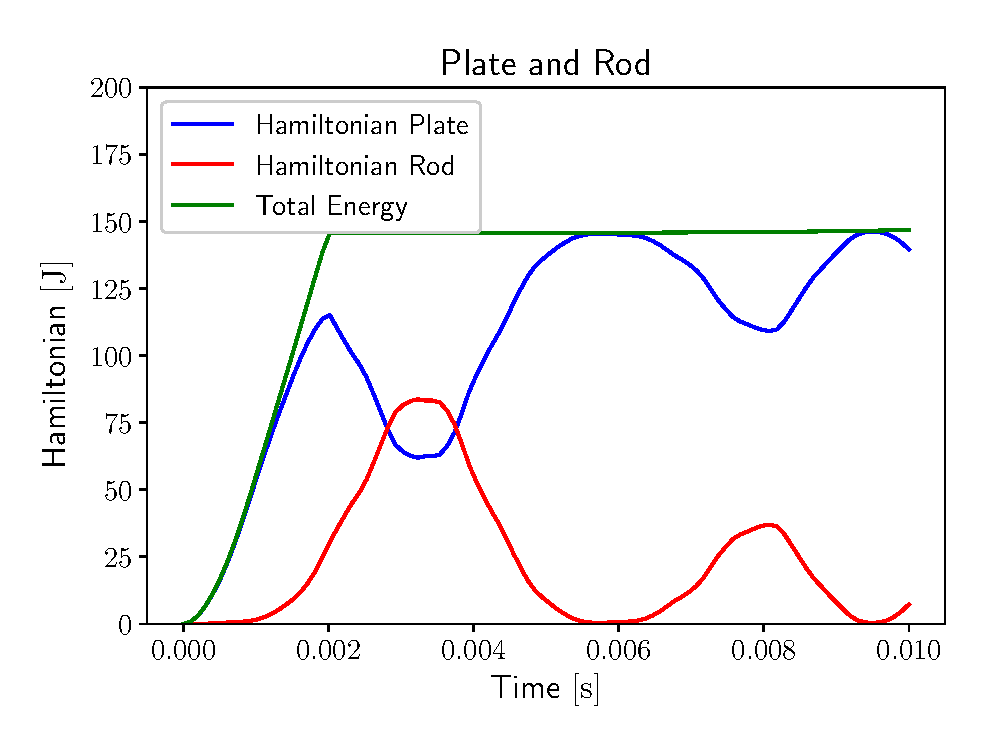
\includegraphics[width=0.48\textwidth]{HamiltonianRod.eps}
		}
		
	\end{frame}
	
	
	
	\begin{frame}{Irrotational Shallow Water Equations}
		
		\only<1>{
			\begin{center}
				\includemedia[
				label=vidDam,
				addresource=/home/andrea/Videos/Videos_defense/Saint_Venant_nobar.mp4,
				activate=pageopen,
				width=10cm, height=5cm,
				flashvars={
					source=/home/andrea/Videos/Videos_defense/Saint_Venant_nobar.mp4
					&loop=true
				}
				]{}{VPlayer.swf}
				
				\mediabutton[
				mediacommand=vidDam:playPause,
				]{\fbox{Play/Pause}}
				
			\end{center}
		}
		
		\only<2>{
			\begin{center}
				\includegraphics[width=0.48\textwidth]{Hamiltonian_SWE.eps}
				\includegraphics[width=0.48\textwidth]{Lyapunov_SWE.eps}
			\end{center}
		}
	\end{frame}


\begin{frame}{Multibody vibration}
	\only<1>{
		\begin{figure}
			\centering
			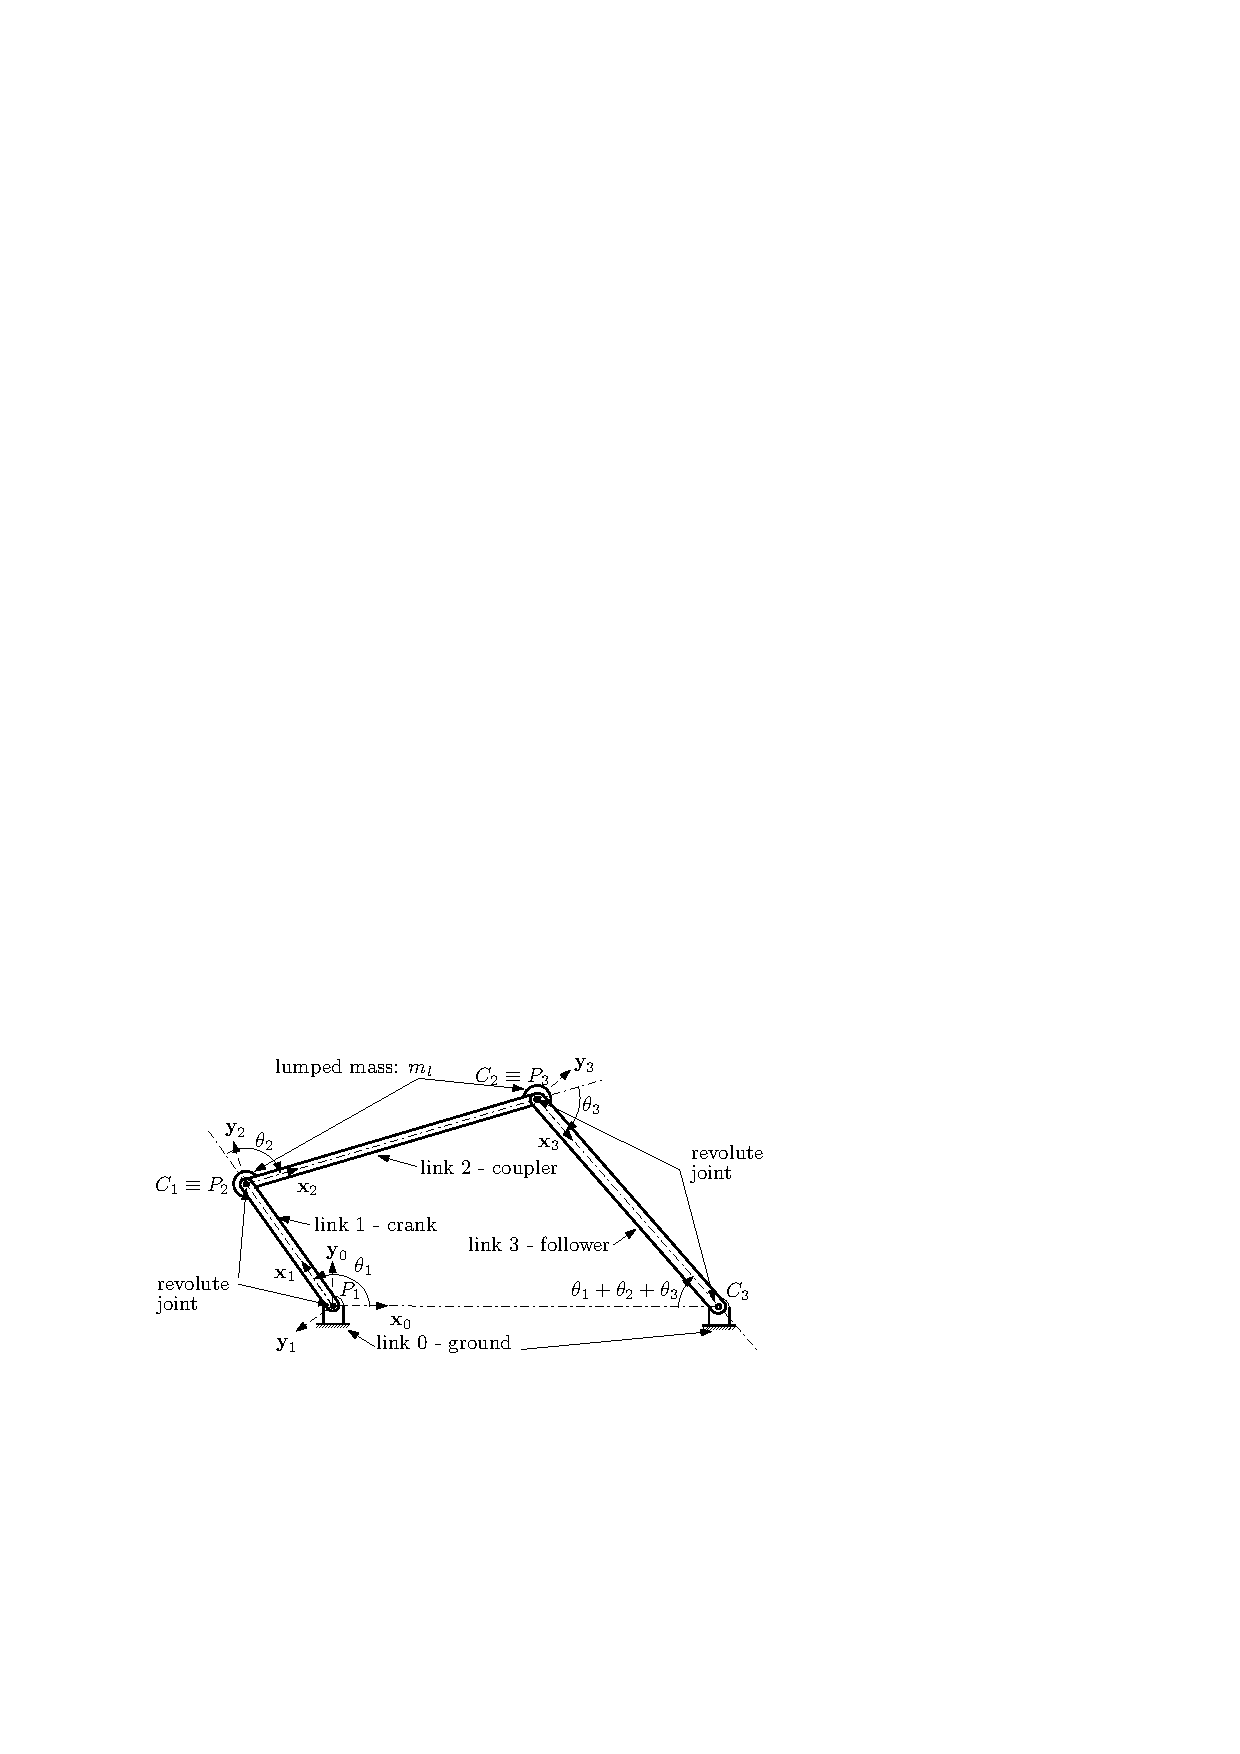
\includegraphics[width=0.7\textwidth]{fourbars.pdf}
		\end{figure}	
	}
	\only<2>{
		\begin{figure}
			\centering
			\includegraphics[width=0.4\textwidth]{block_4bars.eps}
		\end{figure}	
	}
	\only<3>{
		\begin{figure}
			\centering
			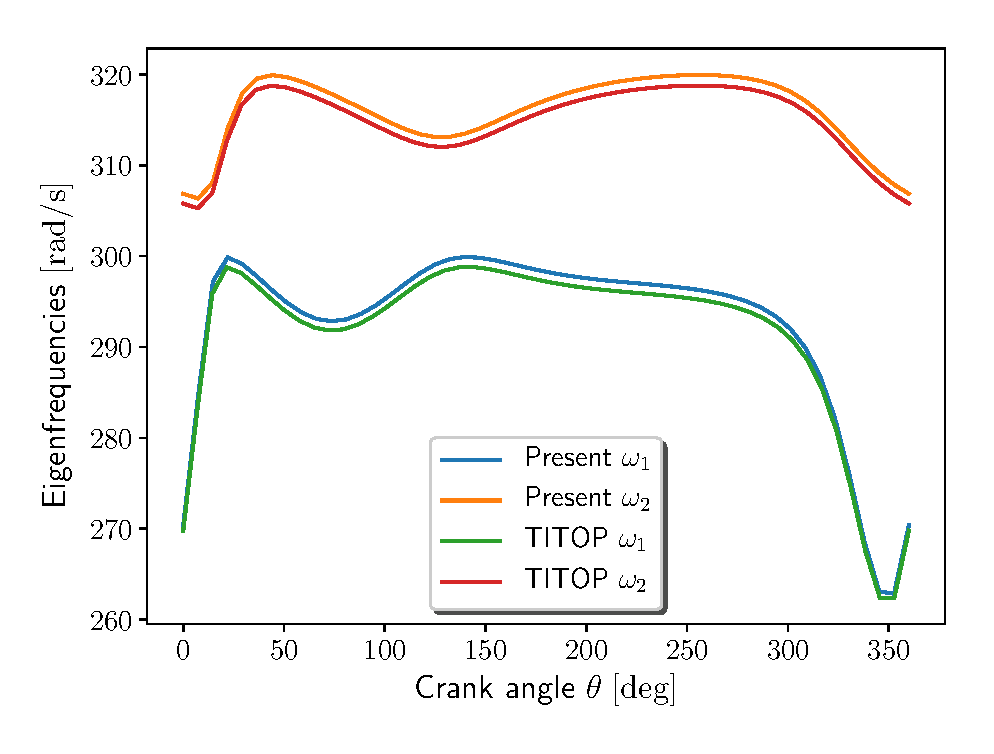
\includegraphics[width=.7\textwidth]{FourBar_Om12_Chebbi.eps}
		\end{figure}	
	}
\end{frame}

\begin{frame}{Taylor Green Vortex}
	\begin{center}
		\includemedia[
	label=vidTG2D,
	addresource=/home/andrea/Videos/CandidatureISAE/vorticityTG2D.mp4,
	activate=pageopen, 
	deactivate=onclick,
	width=9cm, height=6cm,
	flashvars={
		source=/home/andrea/Videos/CandidatureISAE/vorticityTG2D.mp4&%
		autoPlay=true&%
		loop=true%
	}
	]{}{VPlayer.swf}
	%\mediabutton[
	%mediacommand=vidTG2D:playPause
	%]{\fbox{Play/Pause}}
	\end{center}

\end{frame}
	
\begin{frame}{3D Maxwell equations}
	\begin{center}
\includemedia[
label=vidMaxwell3D,
addresource=/home/andrea/Videos/CandidatureISAE/MaxwellE13D.mp4,
activate=pageopen, 
deactivate=onclick,
width=9cm, height=6cm,
flashvars={
	source=/home/andrea/Videos/CandidatureISAE/MaxwellE13D.mp4
	&%
	autoPlay=true&%
	loop=true%
}
]{}{VPlayer.swf}
%\mediabutton[
%mediacommand=vidMaxwell3D:playPause,
%]{\fbox{Play/Pause}}
	\end{center}
	
\end{frame}

	
	\section{Portwings Activity}
	
	
	\begin{frame}{Exterior calculus and discretization of PDEs}
		
		\begin{block}{A unified discretization framework}
		\textit{"Just as the arrangement of the chemical elements in a periodic table led to the discovery of new elements, the periodic table of finite elements has not only clarified existing elements but also highlighted holes in our knowledge and led to new families of finite elements suited for certain purposes."}
		\end{block}
	\begin{figure}[t]
			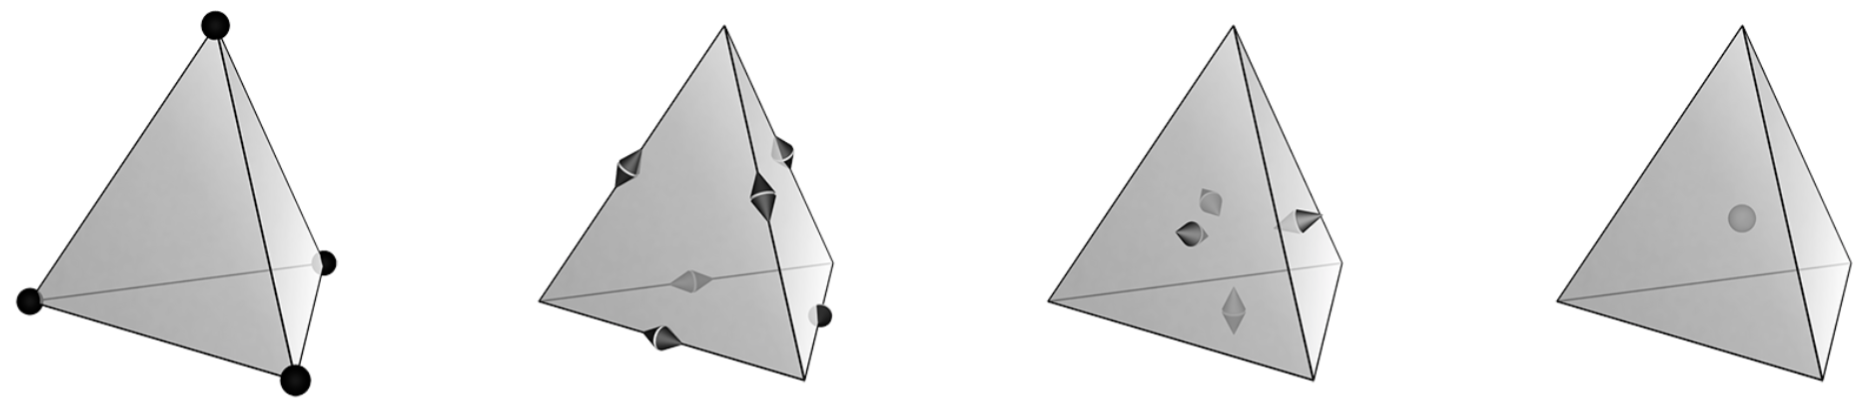
\includegraphics[width=\columnwidth]{Whitney.png}%
	\end{figure}
		
	\end{frame}
	
	
	\section{Why pH is any better?}
	
	
	\begin{frame}{The irreducible wave equation}
		From the linearization of mass and momentum conservation, the acoustic wave equation in irreducible form is obtained
		\begin{equation*}
			\frac{1}{\kappa} \diffp[2]{p}{t} - \div\left(\frac{1}{\rho}\grad p\right) = 0,  \qquad \bm{x} \in \Omega \subset \bbR^3, \quad p|_{\partial\Omega} =0,
		\end{equation*}
		$p$ is the pressure, $\rho$ the density and $\kappa$ the bulk modulus.
		
		
		\begin{block}{The standard discretization}
			Standard continuous Galerkin scheme:
			\begin{equation*}
				\mathbf{M}_{\kappa^{-1}} \ddot{\mathbf{p}} + \mathbf{K}_{\rho^{-1}} \mathbf{p} = \mathbf{0}.
			\end{equation*}
			What about conservation of energy? Yes, \textcolor{red}{but a Newmark scheme is needed}.\\
			Mass and momentum conservation? \textcolor{red}{Lost (additional analysis required)}.
		\end{block}
		
	\end{frame}
	
	\begin{frame}{Maybe the reduction went too far}
		\begin{overlayarea}{\textwidth}{\textheight}
			Consider two auxiliary variables
			\begin{equation*}
				v = \partial_t p, \qquad  \bm{\sigma} = \rho^{-1} \grad p, \qquad (v \text{ satisfies } v|_{\partial \Omega}=0),
			\end{equation*}
				two coupled conservation laws (mass and momentum) are obtained
				\begin{equation*}
					\begin{bmatrix}
						\kappa^{-1} & 0 \\
						\bm{0} & \rho 
					\end{bmatrix} \diffp{}{t}
					\begin{pmatrix}
						v \\ \bm{\sigma}
					\end{pmatrix} = 
					\begin{bmatrix}
						0 & \div \\
						\grad & \bm{0}
					\end{bmatrix}
					\begin{pmatrix}
						v \\ \bm{\sigma}
					\end{pmatrix}.
				\end{equation*}
				This system is an Hamiltonian reformulation.
			

		\end{overlayarea}
	\end{frame}
	
	\begin{frame}{The mixed finite element (partial) solution}
		\begin{overlayarea}{\textwidth}{\textheight}
			
			\only<1>{
				\begin{block}{Mixed $\div$ formulation}
					Find $v_h \in V_h^3, \; \bm{\sigma}_h \in \Sigma_h^2$ such that
					\begin{equation*}
						\begin{aligned}
							\inpr[\Omega]{\psi_v}{\kappa^{-1}\partial_t v_h} &= +\inpr[\Omega]{ \psi_v}{\div\bm{\sigma}_h}, \\
							\inpr[\Omega]{\bm{\psi}_\sigma}{\rho \partial_t \bm{\sigma}_h} &= -\inpr[\Omega]{\div\bm{\psi}_\sigma}{v_h}, \\
						\end{aligned} \qquad
						\begin{aligned}
							\forall \psi_v &\in  V_h^3, \\
							\forall \bm{\psi}_\sigma &\in \Sigma_h^2 \\
						\end{aligned}
					\end{equation*}
					Properties of the numerical algorithm:
					\begin{itemize}
						\item[\textcolor{green}{\checkmark}] Symplectic schemes guarantee discrete energy conservation;
						\item[\textcolor{green}{\checkmark}] Discrete mass conservation 
						\begin{equation*}
							\kappa^{-1} \partial v_h = \div \bm{\sigma_h}
						\end{equation*}
						\item[\textcolor{red}{$\times$}] No momentum conservation;
					\end{itemize}
				\end{block}
			}
			
			\only<2>{
				\begin{block}{Mixed $\grad$ formulation}
					Find $v_h \in V_h^0, \; \bm{\sigma}_h \in \Sigma_h^1$ such that
					\begin{equation*}
						\begin{aligned}
							\inpr[\Omega]{\psi_v}{\kappa^{-1}\partial_t v_h} &= -\inpr[\Omega]{\grad \psi_v}{\bm{\sigma}_h}, \\
							\inpr[\Omega]{\bm{\psi}_\sigma}{\rho \partial_t \bm{\sigma}_h} &= +\inpr[\Omega]{ \bm{\psi}_\sigma}{\grad v_h}, \\
						\end{aligned} \qquad
						\begin{aligned}
							\forall \psi_v &\in V_h^0, \\
							\forall \bm{\psi}_\sigma &\in \Sigma_h^1. \\
						\end{aligned}
					\end{equation*}

					Properties of the numerical algorithm:
					\begin{itemize}
						\item[\textcolor{green}{\checkmark}] Symplectic schemes guarantee discrete energy conservation;
						\item[\textcolor{green}{\checkmark}] Discrete momentum conservation
						\begin{equation*}
							\rho \partial_t \bm{\sigma_h} = \grad v_h .
						\end{equation*}
						\item[\textcolor{red}{$\times$}] No mass conservation;
					\end{itemize}
				\end{block}
				
				\Large{Conservation laws cannot be both satisfied!}
			}
			
			
		\end{overlayarea}
	\end{frame}
	
	
	\begin{frame}{Geometric discretization and pH systems}
		Combining the two previous formulations, one replicates the topological and physical properties of the system numerically.
	
			\begin{tcolorbox}
				\begin{itemize}
					\item Numerical stability by construction;
					\item Conserve mass, momentum, energy;
					\item Enforces power continuity in the domain and at the boundary.
				\end{itemize}
			\end{tcolorbox}
		
	\end{frame}
	
	
\end{document}